\chapter{Implementation}
\label{chapter:implementation}
\section{Option Pricing}
\label{section:Option Pricing}
The theoretical models presented in Chapter \ref{chapter:background} attempt to model the movements of real-world stock prices. With these predictions, we should be able to better replicate real option prices than if we assumed a simple constant volatility.

Currently, the two most used methods to computationally price options are known as \emph{finite differences}~\cite{Hull} and \emph{Monte Carlo}~\cite{Glasserman}.

Finite differences is an extremely fast procedure when used to price either European or American-type options, making it very appealing in these circumstances. However, when used to price other option types whose value depends on the stock prices until maturity (e.g. Asian options), the algorithm becomes very slow, rendering it almost useless.
The implementation of both Heston and SABR models (presented before) using finite differences can be found in deGraaf~\cite{deGraaf}.


With the Monte Carlo algorithm, we begin by simulating a very large number of stock price paths (e.g. 100,000 simulations). The option's payoff is then calculated for each of these simulated paths and averaged, providing a fair estimate of the option's value. This algorithm can also be easily adapted to price exotic options, making it very attractive in such cases.
In the past, simulating all the stock price paths took prohibitively long computation times and this method was often discarded for this reason. However, with the recent advancements in computer hardware and new algorithmic developments, such as GPU implementation, this method has become quite popular.
For these reasons, the Monte Carlo method will be used for the analysis of the models presented before.


\subsection{Simulating stock prices}
\label{subsection:Simulating stock prices}
As stated, to implement the Monte Carlo algorithm, one needs to simulate stock price paths. However, by analyzing eq.\eqref{GBM}, we can see that the stock prices depend on a Brownian motion process (also known as a Wiener process) which, due to its self-similarity, is not differentiable~\cite{Mikosch}. It follows that stock price paths can never be exactly simulated. Though this exact simulation is impossible, we can approximate the movement of stock price paths by discretizing the Brownian motion process in time, thus solving its self-similarity problem. The two most common discretization procedures are presented below.

\subsubsection{Euler–Maruyama discretization}
\hl{put this in background section?} One of the most well known discretization methods is known as \emph{Euler–Maruyama discretization}, and can be applied to stochastic differential equations of the type
\begin{equation}\label{SDE}
dX(t)=a(X(t))dt+b(X(t))dW(t),
\end{equation}
\noindent where $a(X(t))$ and $b(X(t))$ are some given functions of $X(t)$ and $\{W(t),\ t>0\}$ defines a one-dimensional Brownian motion process.
To apply this discretization, we begin by partitioning the simulation interval $[0,T]$ into $N$ subintervals of width $\Delta t=T/N$ and then recursively define
\begin{equation}
X_{n+1}=X_n+a(X_n)\Delta t+b(X_n)\Delta W_n,
\end{equation}
\noindent for $n=1,\ldots,N$ where $\Delta W_n=W_{t+\Delta t}-W_{t}$.
Using the known properties of Brownian motion processes, we can produce $\Delta W_n\sim \sqrt{\Delta t}Z$, where $Z\sim N(0,1)$ defines a standard normal distribution.

Applying this discretization to the Geometric Brownian motion followed by stock price paths, as seen in eq.\eqref{GBM}, we arrive at
\begin{equation}
S(t+\Delta t)=S(t)+rS(t)\Delta t+\sigma(S(t),t)S(t)\sqrt{\Delta t}Z.
\end{equation}

Due to its simplicity, the Euler–Maruyama discretization method is the most common in the simulation of stock price paths.


\subsubsection{Milstein Discretization}
For stochastic volatility models, such as Heston and SABR, where the volatility itself follows a stochastic differential equation, such as eq.\eqref{SDE}, the Euler–Maruyama discretization may not be sufficiently accurate. In these cases, we can apply the more precise Milstein method~\cite{Milstein}, defined as
\begin{equation}
X_{n+1}=X_n+a(X_n)\Delta t+b(X_n)\Delta W_n+\frac{1}{2}b(X_n)b'(X_n)((\Delta W_n)^2-\Delta t),
\end{equation}
\noindent where $b'(X_n)$ denotes the derivative of $b(X_n)$ w.r.t. $X_n$. Note that when $b'(X_n)=0$, the Milstein method collapses to the simpler Euler–Maruyama discretization.

Applying this discretization to the Heston model, we arrive at
\begin{equation}
S(t+\Delta t)=S(t)+rS(t)\Delta t+S(t)\sqrt{\nu(t)}\sqrt{\Delta t}Z_1+\frac{1}{2}\nu(t)S(t)\Delta t(Z_1^2-1),
\end{equation}
\begin{equation}
\nu(t+\Delta t)=\nu(t)+\kappa(\overline{\nu}-\nu(t))\Delta t+\eta\sqrt{\nu(t)\Delta t}Z_2+\frac{\eta^2}{4}\Delta t(Z_2^2-1),
\end{equation}
\noindent where $Z_1$ and $Z_2$ are two normal random variables with a correlation of $\rho$.


Applying the Milstein discretization to the SABR model results in
\begin{equation}
F(t+\Delta t)=F(t)+\sigma(t)F^\beta(t)\sqrt{\Delta t}Z_1+\frac{\beta}{2}\sigma^2(t)F^{2\beta-1}(t)\Delta t(Z_1^2-1),
\end{equation}
\begin{equation}
\sigma(t+\Delta t)=\sigma(t)+\nu\sigma(t)\sqrt{\Delta t}Z_2+\frac{\nu^2}{2}\sigma(t)\Delta t(Z_2^2-1),
\end{equation}
\noindent where again $Z_1$ and $Z_2$ are two normal random variables with a correlation of $\rho$.

In both models we need to generate the two correlated normal variables, $Z_1$ and $Z_2$, which we can generate from
\begin{equation}\label{normcorr}
\begin{split}
&Z_1\sim N(0,1);\\
&Z_2=\rho Z_1+\sqrt{1-\rho^2}Y,
\end{split}
\end{equation}
\noindent where $Y\sim N(0,1)$ is uncorrelated with $Z_1$.

Because it is more precise, the Milstein method will be used in the implementation of both Heston and SABR stochastic volatility models. The simpler Euler–Maruyama discretization will be assumed for both constant and Dupire's local volatility.


\subsection{Pricing options from simulations}
\hl{this should come before the discretization methods?}
To price options, we generate $M$ paths by recursively calculating $\{S_i(t),\ \ i=1,\ldots,M\}$ (or $F_i(t)$ in the case of SABR), using either of the discretization methods presented before.

When the stock price at the maturity, $S_i(T)$ (or $F_i(T)=S_i(T)$), is obtained, the option's payoff for each path is calculated from eq.\eqref{callput}. We then average all these results and discount them to the present, obtaining the (call) option's value
\begin{equation}
C(K,T)=e^{-rT}\frac{1}{M}\sum_{i=1}^M\max\left(S_i(T)-K,0\right).
\end{equation}

It is important to note that, the smaller our subintervals $\Delta t$ are, the better is the approximation done when discretizing the Brownian motion process. However, by decreasing $\Delta t$ we increase the number of intervals and with it the number of calculations needed to obtain each $S_i(T)$. The compromise between computation time and precision must be handled appropriately.
 \hl{put some image here to exemplify the different time steps dt}



\iffalse
depend on a Brownian motion process, it follows that it is not differentiable. For this reason, it's impossible to exactly simulate such a process. An approximation is possible, however, using discrete jumps of length $\Delta t$ and using the Brownian motion property $W(t)\sim \sqrt{t}N(0,1)$~\cite{Mikosch}, with $N(0,1)$ being a normal distribution with 0 expected value and 1 variance.
We can then simply discretize eq. \eqref{BS} into
\begin{equation}
S(t+\Delta t)=S(t)+rS(t)\Delta t+\sqrt{\Delta t}\sigma S(t)N(0,1),
\end{equation}
\noindent where $\Delta t$ corresponds to a given time step. An example of this discretization is illustrated in \autoref{fig:GBM} with the realization of three sample paths.

\begin{figure}[H]
    \centering
      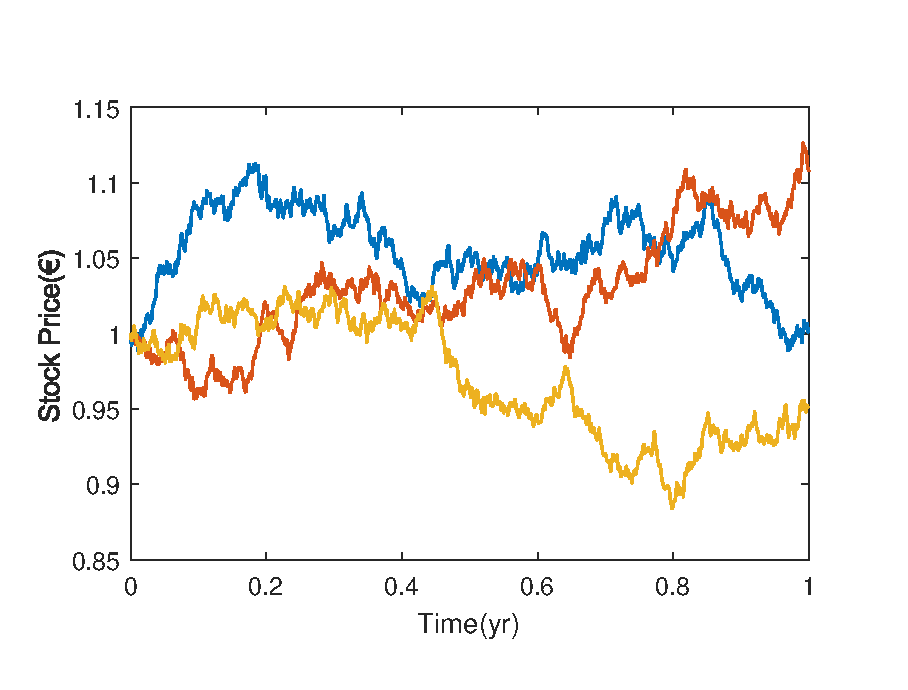
\includegraphics[width=0.9\columnwidth]{GBM.eps}
      \caption{Example of three GBM processes, using the parameters $r=\SI{0.06}{\per\year}$, $\sigma=0.05$, $S(0)=\SI{1}[\EUR]{}$ and time steps $\Delta t=10^{-3}\SI{}{\year}$.}\label{fig:GBM}
    \end{figure}
    
By simulating a large number of paths, some underlying tendencies might become apparent, which will prove useful in option pricing.


 American options, however, pose a much greater challenge.  Unlike European options, no analytic pricing model currently exists for this type of derivatives. Several numerical models have been proposed in the past in an attempt to solve this problem~\cite{Wilmott1,Hull}, such as the Longstaff-Schwartz algorithm~\citep{Longstaff}, which we shall approach in later sections of the present thesis.
\fi 

 
 
 
\section{Model Calibration}
\label{section:Model Calibration}
Both SABR and Heston stochastic volatility models contain variables that need to be calibrated in order to appropriately replicate market option prices.

Calibrating the models' parameters means finding the optimal values for these parameters such that the difference between the prices of market options and options priced under the models' assumptions is minimized. This difference should be measured with a cost function such as
\begin{equation}\label{cost}
\mathrm{Cost}(\theta)=\sum_{i=1}^n\sum_{j=1}^m\left(\frac{C_{\mathrm{model}}(\theta,T_i,K_j)-C_{\mathrm{market}}(T_i,K_j)}{C_{\mathrm{market}}(T_i,K_j)}\right)^2,
\end{equation}
\noindent where we denote $\theta$ as the model's parameter set and $C_{\mathrm{model}}(\cdot)$ and $C_{\mathrm{market}}(\cdot)$ correspond to the model and market option prices, respectively, for maturities $T_i,(i=1,\ldots,n)$ and strikes $K_j,(j=1,\ldots,m)$.

\subsection{Optimization Algorithms}
\subsubsection{Deterministic optimizer}
There are several possible methods to find the minimum value for the cost function shown in eq.\eqref{cost}. In general, most procedures require some initial guess at the parameters' optimal values, $\theta_0$. The cost function for these values, $\mathrm{Cost}(\theta)$, is calculated. A new parameter vector, $\theta'$, is then generated in the neighborhood of the starting point and the cost function is recalculated, $\mathrm{Cost}(\theta')$. If the error decreases with this new vector (i.e. $\mathrm{Cost}(\theta')<\mathrm{Cost}(\theta)$), the new parameter values are assumed - otherwise they are discarded. This procedure is repeated until the cost function decreases below a threshold.
This algorithm is called deterministic because if we run the optimization twice with the same initial guess, the minima found in both instances will be the same.

This method is systematized in Algorithm \ref{DetOpt}.

\begin{algorithm}[H]\label{DetOpt}
\DontPrintSemicolon
 Define $\theta=\theta_0$\tcc*[r]{Initial guess}
 \While{$\mathrm{Cost}(\theta)>\mathrm{Threshold}$}{
  Generate $\theta'$\tcc*[r]{New parameter vector}
  \If{$\mathrm{Cost}(\theta)>\mathrm{Cost}(\theta')$}{
   $\theta=\theta'$\;
   }
 }
 Optimal parameters: $\theta^{*}=\theta$\;
 \caption{Deterministic Optimizer}
\end{algorithm}
\ 

The main problem with this algorithm is the fact that the cost function may be nonlinear, meaning that it might contain several local minima. This is problematic because the optimization procedure will only progress in directions where the cost function decreases and it may get stuck in these points meaning that the global minimum will not be reached.
The minimum found by the algorithm is expected to be heavily dependent on our initial guess, which is very undesirable.


Two possible workarounds exist around this problem, which we will refer to as \emph{multi-start optimizer} and \emph{stochastic optimizer}.

\subsubsection{Multi-Start Optimizer}
With the multi-start optimizer we run the deterministic optimization algorithm (described before) for a set of different starting points. Several local optima will be found on all the instances of the local optimizer and we select the one where the cost function is minimal.

This procedure is depicted in Algorithm \ref{MSOpt}.

\begin{algorithm}[H]\label{MSOpt}
\DontPrintSemicolon
Generate $\theta_{0,i},\ \ i=1,\ldots,N$\tcc*[r]{Multiple starting points}
 \For{$i=1,\ldots,N$}{
  Run Algorithm \ref{DetOpt} with initial guess $\theta_{0,i}$\;
  Calculate $\mathrm{Cost}(\theta_i')$ for the obtained minima $\theta_i'$\;
 }
 Optimal parameters: $\theta^{*}=\underset{\theta_i'}{\arg\min}\left\{\mathrm{Cost}(\theta_i')\right\}$\;
 \caption{Multi-Start Optimizer}
\end{algorithm}
\ 


\subsubsection{Stochastic Optimizer}
As for the stochastic optimizer, the algorithm  starts with the initial guess, $\theta_0$, and calculates its cost function $\mathrm{Cost}(\theta)$. Like the deterministic optimizer (Algorithm \ref{DetOpt}), it picks a new vector, $theta'$, in the neighborhood of the first and calculates its cost function, $\mathrm{Cost}(\theta')$. Before, with deterministic optimizer, this new vector would be accepted only if the cost function had decreased. However, with the stochastic optimizer there is a chance, defined by an acceptance probability function $P(\mathrm{Cost}(\theta),\mathrm{Cost}(\theta'))$, that the new vector is accepted even if the cost function increases. Thus, if the optimizer gets stuck at a local minimum, it may be able to escape from it until, ideally, the global optimum is found. One example of such algorithms is known as simulated annealing. An appropriate acceptance probability function must be found for the optimization.


This method is represented in Algorithm \ref{StochOpt}.

\begin{algorithm}[H]\label{StochOpt}
\DontPrintSemicolon
 Define $\theta=\theta_0$\tcc*[r]{Initial guess}
 \While{$\mathrm{Cost}(\theta)>\mathrm{Threshold}$}{
 Generate $\theta'$\tcc*[r]{New parameter vector}
  \If(\tcc*[f]{Acceptance Probability Function}){$P(\mathrm{Cost}(\theta),\mathrm{Cost}(\theta'))<\mathrm{random}(0,1)$}{Set $\theta=\theta'$\;}  
 }
 Optimal parameters: $\theta^{*}=\theta$\;
 \caption{Stochastic Optimizer}
\end{algorithm}
\ 


\subsection{Closed Form Solutions and Calibration}
Both optimizers described before require a very large number of model pricer instances to be called. At each iteration, the pricer needs to run once for all maturities and strikes for which we have market data in order to evaluate the cost function. This is extremely problematic if the pricer takes too long to run, since investors demand prices to be produced in a matter of seconds.


The main reason why Heston and SABR are so popular is the fact that both models have closed-form solutions, shown in eqs. \eqref{CH}, \eqref{sabr} and \eqref{dynsabr}. We can use these to directly price the options without the need to run the slow Monte Carlo pricer. The optimization algorithm should then converge much faster, enabling us to use the slower stochastic optimization algorithms to reach the global optimum.





